\chapter{INTRODUÇÃO}

\section{JUSTIFICATIVA}

Acredita-se que o campo de trabalho para os novos dos profissionais atuantes na área das ciências agrárias tem mudado, a busca pela valorização das capacidades e competências ocupacionais. Busca-se cada vez mais a afirmação e promoção de direitos de cidadania, associatividade política, responsabilidade social e ambiental, consideração, respeito as diversidades étnicas e culturais que devem ser valorizadas constantemente, para tal, a academia  tem um papel importante neste contexto, que é  o de fomentar e oportunizar essas competências. Dentro deste contexto a capacidade de manter-se fio a inovação, especialmente a destrutiva é fundamental ao progresso do crescimento e manutenção futura do profissional das agrárias no novo mercado de serviços e produtos, assim como saber lidar com os novos empreendimentos nos campos de atuação.

De acordo com \citeonline{tarapanoff_monitoramento_2016}, existe um cenário favorável para os negócios rurais que buscam a sustentabilidade econômica e ambiental. Nesse sentido o Brasil deve buscar trilhar  um caminho seguro em relação à sustentabilidade de seu agronegócio, em consonância com as melhores práticas da exploração ambiental e a produção agrícola, parte promovida por cumprimentos a regras ambientais a exemplo a Agenda 2030 que prevê a exploração consciente dos recursos naturais e tomando medidas urgentes sobre a mudanças climáticas individuais quanto institucionais, \cite{filho_documentos_2017}.

O desenvolvimento sustentável pode ser definido segundo \cite{lara_ideologia_2017} como um negócio socialmente responsável e ecologicamente correto, mas invariavelmente viável em termos financeiros. Concomitantemente existe uma lacuna na formação profissional durante o ensino superior no que se refere à adoção de uma cultura empreendedora, \cite{lima_ser_2015}. Não tem sido possibilitado aos acadêmicos, a oportunidade de gerar inovação tecnológica sustentável, inclusive para a aplicação prática dos conhecimentos adquiridos. Da mesma maneira, para que para uma ideia inovadora alcance o sucesso desejado é preciso muito mais que o conhecimento técnico.Deve ser disponibilizado aos futuros profissionais/empreendedores, treinamento na formulação das ideias em etapas direcionadas e adequadamente orientadas.

Para que um negócio sustentável possa ter sucesso é preciso mais do que uma ideia inovadora, deve ter o meio e os profissionais capacitados para tal, Relatórios da Fundação Kauffman afirma que as Startups criam uma média de 3 milhões de novas vagas de empregos anualmente e que, estes tipos de empreendimentos serão responsáveis pela criação de 60\% dos empregos no  mundo  \cite{brasil_o_2017}. 
Atualmente estes tipos de  negócios contribuem para o crescimento de diversas regiões geográficas, já que não se expandem apenas em tamanho, mas também em novos locais, além de incentivar o emprego em suas indústrias relacionadas. Supletivamente, como muitas dessas microempresas são responsáveis por desenvolver novas tecnologias e processos, elas também geram aumento de absorção do capital humano mais capacitado para gerenciamento empresarial.

Diante deste cenário, para que o aprendizado dos profissionais seja mais efetivo, surgem diversas abordagens e metodologias a serem assimiladas. Nesse contexto, deve existir uma maior produção de estudos e conteúdos sobre o empreendedorismo e os modelos educacionais que melhor se apliquem ao aprendizado deste, como ressalta \citeonline{kuratako_entrepreneurship_2003}. É notória a urgência de se pesquisar o ensino em empreendedorismo de forma disciplinada no meio acadêmico. Por ser um tema de grande importância, a educação empreendedora promovida no seio do ensino superior pode ser o caminho para o surgimento de inovações sustentáveis e economicamente viáveis passives e escaláveis.

Dentro do contexto metodológico educacional, temos as metodologias ativas, que trazem a possibilidade de mudança da centralidade no docente (ensino) para o estudante (aprendizagem), ponto de vista preconizado por \citeonline{freire_pedagogia_1987} ao abordar educação como um processo que não é realizado por outrem, ou pelo próprio indivíduo, mas que acontece na interação entre pessoas através de sua vivência por palavras, ações e reflexões. 
Enquanto o método tradicional de ensino utiliza a transmissão de informações e concentra as atividades no docente, na metodologia ativa, os alunos ocupam a centralidade da educação e o conhecimento é construído de forma colaborativa. Sucintamente, as metodologias ativas propõem transformar o processo de ensiagem na busca pelo comportamento empreendedor, como uma forma de enfrentar o modelo tradicional praticado e aceito ao longo dos anos.
 
As práticas ativas estimulam o reconhecimento das dificuldades do mundo atual, tornando os alunos aptos a intervir na promoção das transformações necessárias a exemplo as que se baseiam  na reflexão e argumentação \cite{bezanilla_methodologies_2019}. Assim, o aluno torna-se protagonista da sua aprendizagem e autônomo no alcance dos seus objetivos incorporando seus valores e razões \cite{rubel_student_2016}. Existem vários recursos, métodos e técnicas para alcançar o satisfatório comportamento empreendedor, como: uso de tecnologias digitais e aplicativos \cite{pereira_use_2020}, ensino híbrido e suas estratégias como sala de aula em rotação por estações, Aprendizagem Baseada em Problemas (ABP) \cite{souza_aprendizagem_2015}, e uso de situações-problema e estudos de hipóteses problemas, sala de aula invertida \cite{junior_sala_2016,branco_sala_2016}, uso de mapas mentais \cite{junior_percepcao_2018}, sala de aula compartilhada \cite{strack_por_2009}, estratégias de Design Thinking \cite{andrews_circular_2015}, Gamificação \cite{ogawa_avaliacao_2016}, projetos de extensão \cite{garcia_contribuicao_2012}, dentre tantos outros recursos do método ativo, os quais podem vir facilitar o entendimento e a compressão dos acadêmicos das Ciências Agrárias no contexto de um mercado de trabalho que se apresenta com um perfil voltado ao empreendedor.

O empreendedorismo é a habilidade de reunir esforços para transformar em realidade uma oportunidade, objetivando a satisfação pessoal do empreendedor e o lucro. Tal conceito define o empreendedorismo como uma prática constante das atividades rotineiras dos educandos. Desde a capacidade de resolução de problemas quanto a idealização de propostas capazes de inovar. Dentro desta dicotomia entre empreendedorismo e educação surge a "Educação Empreendedora", que construída por práticas e dinâmicas idealizadas, buscando a melhoria na promoção do comportamento empreendedor \cite{martins_educacao_2016, morais_empreendedorismo_2018}, e resolução de problemas de forma sustentável e rápida.

É diante desta problemática que este projeto busca avaliar a inovação sustentável e a eficácia da promoção empreendedora por uma ação de educação tendo em conta aos negócios rurais, pelo Programa Empreenda Agro Sustentável promovido para os acadêmicos das ciências agrárias, utilizando para este fim, Workshops encadeados e ferramentas didáticas que buscam capacita-los para a construção de propostas inovadoras viáveis.


\section{DELIMITAÇÕES DO ESTUDO}

Esta pesquisa está focada na dissonância entre a teoria e prática dos métodos educacionais e as mudanças vertiginosas do mercado de trabalho no meio rural. Este Setor foi escolhido por estar contribuindo significativamente para a balança comercial do país, apresentando saldos positivos frequentes. Igualmente contribui, para a segurança alimentar do País e produção de produtos limpos e renováveis. O mercado emergente apresenta significativa contribuição para a empregabilidade da população no campo, invertendo cada vez mais o êxodo rural, porém, este mercado que absorve novos profissionais, exige que tais profissionais se mostrem a cada dia mais capacitados para lidar com o desenvolvimento tecnológico e a produção em larga escala, em que a busca pela valorização das capacidades e competências profissionais aumenta a cada dia. 

Em contraponto o empreendedorismo atualmente se confunde com a Meritocracia. Tantos a meritocracia quanto o empreendedorismo caminham juntos no cerne do movimento de individualização no mundo do trabalho \cite{costa_novo_2019}. Os dois  Projetam imagens individuais de trabalho e sucesso, em que a capacidade individual somada as oportunidades geram resultados positivos junto ao mercado de trabalho. Porém, o Empreendedorismo derivado da educação empreendedora, proposto neste projeto, surge atrelado a técnicas e métodos capazes de facilitar e validar as propostas empreendedoras, assim sendo um programa que vise o incentivo as práticas empreendedoras de forma sistemática e coerentes distingue dos resultados negativos que estão atrelados a meritocracia e suas vantagens a frente dos pares distintos.

Visando compreender o comportamento empreendedor nos alunos dos cursos do Centro Ciências Agrárias Aplicadas CCAA da Universidade Federal de Sergipe-UFS, foi escolhida a população para esta pesquisa de 1.453 discentes dos cursos de graduação nas áreas de agrárias da Universidade Federal de Sergipe (UFS): Engenharia Agronômica, Engenharia Agrícola, Zootecnia, Engenharia Florestal, Veterinária e Engenharia de Pesca, dados contidos no relatório estatístico de matrículas 2017 da instituição. A amostra compreenderá  120 discentes que participarem do programa Empreenda Agro Sustentável.

As atividades serão desenvolvidas por quatro workshops, que constam metodologias ativas, oficinas, palestras tendo em conta a promoção da aprendizagem significativa e colaborativa. Durante os módulos do projeto (workshops), os participantes testarão de seus \textit{insights} para que novas requisições sejam realizadas e/ou que erros nos planejamentos sejam encontrados e, consequentemente, debatidos e mitigados. Depois que todas as \textit{Sprints} (atividades dos três workshops) forem finalizadas, ou seja, que todos os módulos sejam abordados, será iniciado um ciclo de Apresentações e desenvolvimento da habilidade de apresentação e demonstração dos produtos por apresentações sumárias (Pitchs). O programa será desenvolvido em quatro encontros "workshops", que abordarão temas pertencentes ao empreendedorismo e o comportamento empreendedor, a saber: 

\begin{itemize}

\item {1º Workshop: O que é startups, empreendedorismo, comportamento empreendedor e cultura empreendedora, problemas (segmentação do mercado), segundo os Objetivos do Desenvolvimento Sustentável (ODS), Modelagem do negócio e Criatividade;}
\item {2º Workshop: A busca de oportunidades como característica empreendedora, construção do \textit{Lean Canvas}, mapa de empatia, validação da proposta de valor, economia colaborativa e \textit{coworking};}

\item {3º Workshop: Makeathon: Prototipagem para o MCVP, O que você pode fazer por seu cliente e como o cliente adquire seu produto?;}
\item {4º Workshop: Demoday. Destaca-se que o mecanismo de pesquisa que será utilizado neste experimento foi composto por Cinco blocos de questões de múltipla escolha baseadas principalmente em escalas de cinco ou sete possibilidades.}
\end{itemize}

O  primeiro conjunto de questões está relacionado a informações que buscam traçar o perfil dos alunos entrevistados, tais como: gênero, faixa etária, curso vinculado e o perfil de interesse nas áreas de estudo ligadas ao empreendedorismo sustentável tal questionário foi baseado no trabalho desenvolvido por \citeonline{lima_ser_2015}. O segundo bloco e composto por 10 questões relacionadas a autoeficácia dos estudantes de múltipla escolha partindo da alternativa “Completamente Inseguro” a "Completamente Seguro”. O terceiro bloco e composto por 7 questões que analisam a intenção empreendedora do aluno da quais segue uma proporção partindo da resposta, tendo como alternativas, partido do “Discordo totalmente” a “Concordo totalmente”. O Quarto bloco retrata a intensão ter sua própria empresa ou ser autônomo e por fim, o quinto bloco contendo 11 questões sobre a ligação da família e o apoio familiar no empreendedorismo, tendo como alternativas, iniciando no “Discordo totalmente” até o “Concordo totalmente”. Buscando aferir os resultados do programa, um novo questionário abordando as mesmas temáticas serão aplicadas ao final do programa. 
O estudo caracteriza-se como uma pesquisa de levantamento ou Survey, que se destaca por compreender uma amostra expressiva em relação ao universo pesquisado. Optou-se por adotar a oportunidade qualitativa para a análise dos dados quanto a percepção do comportamento empreendedor dos alunos, e a abordagem quantitativa na mensuração dos resultados educacionais do Programa Empreenda Agro Sustentável. Após a aplicação dos instrumentos de análise, será realizada a categorização dos dados para que seja possível a classificação da pontuação segundo o questionário GUESS que utilizada testes de hipóteses sobre uma proporção. O projeto traz como benefícios: 

\begin{itemize}
\item{•	Promover o desenvolvimento pessoal, econômico, social no meio rural através da oportunidade de acesso a alternativas de produção de renda;}
\item{Criar a oportunidade de se trabalhar com o que realmente gosta e vencer os entraves do mercado econômico;}
\item{Dar autonomia e liberdade para conduzir o próprio talento, porém, orientado por metodologias específicas;}
\item{Transmitir valores e inspirar novos empreendedores no ambiente agrário;}
\item{Ensinar como lidar com os fracassos e frustrações, sabendo como lós contornar;}
\item{Ensinar estratégias de organização de ideias ou carreiras buscando a receita positiva;}
\end{itemize}


\section{OBJETIVOS}

\subsection{OBJETIVO}

Avaliar o impacto do Programa Empreenda Agro Sustentável como mecanismo indutor da intensão empreendedora para a inovação no setor do agronegócio junto aos acadêmicos das Ciências Agrárias da UFS.



\subsection{OBJETIVOS ESPECÍFICOS}

\begin{itemize}
\item{Identificar o efeito da promoção de iniciação empreendedora, direcionado a inovação sustentável no meio acadêmico;}
\item {Avaliar o potencial empreendedor dos alunos do Centro de Ciências Agrárias Aplicadas participantes do Programa;
}
\item {Fomentar por meio do projeto de extensão o comportamento empreendedor nos alunos do Centro de Ciências Agrárias Aplicadas;}

\item {Tipificar e analisar os tipos de PI que surgem com o incentivo ao empreendedorismo sustentável por meio da aplicação das metodologias trabalhadas no Programa.}

\end{itemize}


\section{PROBLEMA}

O comportamento empreendedor como indutor de inovação, pode ser estimulado mediante o uso de projetos de extensão universitária como o Programa Empreenda Agro Sustentável? 


\section{HIPÓTESE}

Programas que trabalham a promoção do comportamento empreendedor no meio acadêmico promovem o surgimento de inovação.

%\section{RISCOS}
%\begin{itemize}
%\item{Tomar parte do tempo do entrevistado ao responder ao questionário/entrevista;}
%\item{Risco a segurança dos prontuários;}
%\item{Considerar riscos relacionados à divulgação de imagem, quando houver filmagens ou registros fotográficos;}
%\item{Cansaço ou dispersão ao responder questionários;}
%\end{itemize}





%%%%%%%%%%%%%%%%%%%%%%%%%%%%%%%%%%%%%%%%%%%%%%%%%%%%%%%%%%%%%%%%%%%%%%%%%%%%%%%%%%%%%%%%%%%%%%%%%%%%%%%%%%%%%%%%%%%%%%%%%%%%%%%%%%%%%%%%%%%%%%%%%%%%%%
                                                                 %REFERENCIAL TEÓRICO%                                                                             
%%%%%%%%%%%%%%%%%%%%%%%%%%%%%%%%%%%%%%%%%%%%%%%%%%%%%%%%%%%%%%%%%%%%%%%%%%%%%%%%%%%%%%%%%%%%%%%%%%%%%%%%%%%%%%%%%%%%%%%%%%%%%%%%%%%%%%%%%%%%%%%%%%%%%%



\chapter{REFERENCIAL TEÓRICO}

\section{Desenvolvimento Rural Sustentável}

Definir o desenvolvimento do meio rural sustentável requer um considerável esforço observacional e prático, pois, este ambiente vem sofrendo profundas transformações em suas demandas e necessidades, o desenvolvimento que antes se apresentava majoritariamente como produção de subsistência, hoje dá lugar a um complexo sistema agroindustrial \cite{bastos_determinantes_2018} e social. É importante neste sentindo compreender que definir o desenvolvimento rural com apenas um conceito seria uma proposição simplista do contexto de desenvolvimento rural. Partindo da definição de consequência de ações governamentais definidas por \citeonline{navarro_desenvolvimento_2001} como "ações práticas", este autor descreve que o:

\begin{citacao}
“[...] Desenvolvimento rural, portanto, pode ser analisado a posteriori, neste caso se referindo às análises sobre programas já realizados pelo Estado (em seus diferentes níveis) visando a alterar facetas do mundo rural a partir de objetivos previamente definidos. Mas pode se referir também à elaboração de uma "ação prática".
\end{citacao}

O desenvolvimento rural também pode ser compreendido por um conceito mais regional definido como "Desenvolvimento Local". Tal expressão é recente e deriva de iniciativas de mobilização organização social no sentido de promover uma maior representação dos diferentes atores sociais no processo de desenvolvimento. E que o Estado assume papel de agente facilitador desse processo de descentralização das políticas públicas  para ser democrático, a transparência de suas instituições, o equilíbrio das forças exercidas pelas diferentes correntes de interesse e o compromisso com a qualidade de vida na população afetada \cite{campanhola_diretrizes_2000}. Tal conceito demonstra o espaço rural como um local ideal para a promoção de políticas de inovação e a construção de padrões inovadores na relação entre populações e instâncias públicas, numa tentativa de rompimento com a dominação, que parte de baixo para cima. Neste contexto, surge as Organizações Não Governamentais (ONGs) que buscam garantir a participação da população local, e fazer valer tais mudanças atuando normalmente em ambientes geograficamente mais restritos (região rural, povoados ou municípios), \cite{assis_agricultura_2005, campanhola_diretrizes_2000}.

E por fim, este trabalho está direcionado em estudos relacionados ao Desenvolvimento Rural Sustentável. Anteriormente, o conceito de Desenvolvimento Rural Sustentável era denominado por "Progresso Rural", pois, havia um entendido genérico como sentido parcial e prático de “melhoramento do ambiente” \cite{almeida_da_1995}. Entretanto, torna-se imprescindível destacar que, o desenvolvimento sustentável no meio rural não pode ter suas bases de compreensão apenas no progresso econômico, local ou regional. Se mostra de suma importância entender que para compreender a sustentabilidade é necessário ter um olhar sistêmico que permeie todo o processo, envolvendo diversas dimensões, dentre as quais se destacam a econômica, a sociocultural, a político-institucional e a ambiental \cite{vieira_politica_2015}, a ação de desenvolvimento sustentável é por um lado fruto do desenvolvimento social, por outro lado, esta ação contribui com o desenvolvimento da sociedade de forma autossustentável, ao introduzir inovações anti-predatórias, ao satisfazer demandas específicas tendo como base a economia circular e ao tornar mais densas as redes de cooperação buscando a autossuficiência consciente, satisfazendo as necessidades no presente, sem comprometer a capacidade das gerações futuras de suprir suas próprias necessidades \cite{onu_sustainable_2016}.

No Brasil, o desenvolvimento rural propriamente dito teve início com a política de “Intensificação verde” por meio da revolução verde, plano político que teve força de ação iniciando nos anos 60. Tal política era baseada em subsídios de créditos que buscava o estímulo à produção agrícola em larga escala principalmente de \textit{commodities}, do mesmo modo impulsionava o crescimento do setor de transporte com expansão da malha rodoviária, as políticas de crédito rural, os preços mínimos, as pesquisas e extensão rural \cite{kageyama_o_1990}. Os incentivos e créditos que de fato chegaram ao campo foram em sua maioria, utilizados por empresas de maquinários e de insumos industriais para uso agrícola \cite{strassburg_producao_2015}, impulsionando apenas o aumento da produção em escala industrial, deixando de lado as preocupações com a manutenção dos recursos limitados no campo e a capacidade de escalabilidade dos pequenos produtores.

Tal desenvolvimento teve como ponto positivo o estreitamento das fronteiras entre o meio rural e o meio urbano, tornando-as cada vez mais tênues e difusas \cite{freitas_mudancas_2012}, já que a sociedade civil emerge como protagonista desse processo de construção dos pilares para um desenvolvimento mais responsável e abrangente \cite{de_souza_empreendedorismo_2016}. 

Desta forma, os produtores agrícolas atuais além de suprir as necessidades alimentares da população, se desenvolve ainda mais para produzir particularidades para população urbana, como produtos com maior qualidade, rapidez e efetividade na entrega, volume cada vez maior, entre outras. Atualmente ao pensar em tecnologias inovadoras para o campo, é necessário compreender as necessidades do meio urbano e as possíveis capacidades do meio rural, de maneira que este se mantenha autossustentável em todas as características ambientais, sociais e culturais, sendo de suma importância a compreensão do que de fato venha a ser rural e como construir sua sustentabilidade. As soluções propostas para superar esses desafios devem não apenas considerar a maneira como os alimentos são produzidos, mas também ponderar sobre preocupações sociais, ambientais e econômicas \cite{kamble_achieving_2020}. 

O rural deve ser visto segundo \cite{kageyama_desenvolvimento_2008} como, uma amálgama de práticas heterogêneas, estilos mutuamente contrastantes, tendências de desenvolvimento divergentes, posições hegemônicas e mudanças quase subterrâneas que, a princípio, são praticamente imperceptíveis, mas que, por fim, podem mudar todo o sistema de produção. Compreender a complexidade do rural se faz necessário uma vez que a simples padronização do ambiente é um conceito reducionista do campo, uma maneira concisa do que ocorre no rural \cite{van_der_ploeg_trajetorias_2011}. 

O empreendedorismo é uma das ferramentas possíveis para promoção de desenvolvimento do campo e que considera suas complexidades. Para que seja aplicado corretamente, se faz necessário compreender melhor o empreendedorismo sustentável como também a aplicação prática no meio rural. 

Segundo \citeonline{dornelas_como_2003}, o empreendedorismo significa fazer algo novo, diferente, mudar a situação atual e buscar, de forma incessante, novas possibilidades de negociações, tendo como foco a inovação e a criação de valor, outrossim, \citeonline{leite_aprendizagem_2015} trata o empreendedorismo como  um  processo,  que se concentra em iniciar  e  gerir  empreendimentos,  isto  é,  o conjunto  de  conceitos,  métodos,  instrumentos  e  práticas  relacionadas  com  a criação, implantação  e  gerenciamento de novas  empresas  ou organizações.

Existem diversas definições de empreendedorismo, mas a essência resume-se na inovação, ou seja, criação de algo novo ou modificação de algo buscando uma nova aplicação, empregando os recursos disponíveis de forma criativa, assumindo riscos calculados e buscando oportunidades, é um processo de criação de um negócio de valor com recursos limitados tornando-o capitalizável e economicamente viável \cite{costa_empreendedorismo_2006, stevenson_new_1989, lopes_educacao_2010}. Apesar dessa diversidade conceitual, a ideia de empreendedorismo tem sido predominantemente associada às concepções de progresso e tecnologia usual deixando de lado o campo e nele suas aplicações práticas.  

O intenso debate sobre desenvolvimento da agricultura brasileira de forma sustentável em consonância com assuntos econômicos de interesse nacional torna o tema deste trabalho oportuno e atual, haja vista que a agricultura no Brasil corresponde a 19\% do total das exportações no ano de 2018 \cite{mdic_comex_2019}. Entretanto, este meio de produção convive com a limitação dos recursos naturais \cite{jacobi_meio_1999}, levando ao Estado pensar em políticas públicas que busquem soluções para as demandas tecnológicas surgidas no meio rural, e gerar profissionais capazes de compreender a complexidade da intensa produção no campo mantendo o ritmo constante das mudanças tecnológicas ao mesmo tempo, do uso de limitados recursos naturais \cite{costa_dinamica_2016}.
No alcance desse modelo sustentável, um profissional empreendedor deve ser preparado desde a academia por meio da educação empreendedora de modo que seja capaz de melhorar o desempenho produtivo \cite{da_silva_qualidade_2017}, a capacidade competitiva, a melhoria da segurança alimentar do país \cite{hoffmann_brasil_2014} e, ao mesmo tempo garantir a perpetuação da manutenção do meio ambiente, e não apenas replicar novos padrões de produção e distribuição de bens e serviços e do uso dos recursos naturais, além disso, este profissional deve ser capaz de inovar \cite{morais_empreendedorismo_2018}.

Sobre tais bases, conclui-se que o desenvolvimento do campo de forma tradicional dispõe de poucas hipóteses, além da alternativa de uma prática intensiva em capital e exploração dos recursos naturais, cuja intensificação e amplitude pode levar a escassez dos meios \cite{costa_agrarian_2016}. 




\section{Agritechs}

Atualmente passamos por uma fase muito expressiva da disseminação do empreendedorismo no Brasil e no mundo, tendo como exemplo o crescimento das "Startups" saindo de 2519 em 2012, para 12.815 na presente data, \cite{abstartups_startupbase_2019}. A velocidade do desenvolvimento e conexões das negociações antes realizadas de pessoa a pessoa, atualmente passa pelo campo da automação e digitalização aumentando a velocidade da inovação interferindo na relação entre pessoas e produtividade \cite{campos_o_2016}. 


Independentemente do tamanho e demanda que venha a ter o proprietário do comércio, o desempenho negocial do empreendimento depende da capacidade de adaptação e resiliência  do administrador, assim também são os negócios no meio rural. O grande produtor objetivando o desenvolvimento de capital utiliza-se de um vasto corpo de recursos humanos e tecnológico, já os pequenos produtores muitas vezes dependem apenas deles mesmos, sendo proprietário e administrador, ou quando exige a possibilidade de contratação passa a depender de apenas um profissional responsável por lidar com todos os entraves da produção agrícola e as mudanças constantes do meio rural \cite{soares_relacao_2017}. Uma das alternativas possíveis para reduzir os riscos de se manter em todas as funções citadas em apenas um profissional, é o investimento em tecnologia e inovação tais como: sementes melhoradas, adubação agrícola mais eficiente, centros coletivos de pesquisa direcionadas ao campo (Universidades e empresas) \cite{bochi_dorneles_coletivos_2014, gomes_inovacao_2014} e pequenas empresas prestadoras (startups) de serviços ou nichos do mercado rural. Estes negócios objetivam a melhoria de determinada área agropecuária \cite{junior_agtechs:_2019} ou necessidade do negócio, de forma efetiva e economicamente viável. Elas surgiram por meio das oportunidades que os negócios e as necessidades lhes apresentaram. As Startups transformam as necessidades e ideias em negócio viável e sustentável, ligam-se muito ao meio rural já que para obter sucesso e alcançar o crescimento rápido na produtividade agrícola é necessária uma capacidade de gerar tecnologias adaptativas e ecológicas \cite{contini_hayami_2019}.

O modo como se processa a diversificação tecnológica no campo relaciona-se diretamente com o desenvolvimento e a adaptação de novas tecnologias agrícolas e a diversidade das condições socioeconômicas e ambientais \cite{fen-azmeyer_o_2019}. Neste ambiente de cocriação surge as Startups direcionadas à agricultura, tais empresas de base tecnológica são focadas em soluções para o agronegócio, muitas vezes são referenciadas como um setor \textit{Agtech} \cite{blanco_agtechs:_2019}.

Dentre o espectro de novos empreendimentos, os mais comuns para o agro negócio no Brasil são: \textit{Business to Business} (B2B), \textit{Business to Consumer} (B2C), \textit{Business to Business to Consumer} (B2B2) e o \textit{Direct to Consumer} (D2C). Segundo \citeonline{junior_agtechs:_2019} e \cite{abstartups_startupbase_2019}, as principais  áreas de atuação destas Startups são as áreas de: Biotecnologia de Alimentos inovadores atendendo tanto B2B quanto B2B2C, Marketplace do agronegócio (B2B2C), Bioenergia e Biomateriais (B2B), indústria de Software como Serviço SaaS (B2B).


\section{Comportamento Empreendedor e Educação empreendedora}



Estudos recentes demonstram que a motivação da abertura de negócios vai muito além do dualismo oportunidade-necessidade, ou seja, a criação e/ou descoberta de oportunidades, faz parte também o medo do desemprego, da incapacidade de adaptação as mudanças tecnológicas especialmente em países em desenvolvimento \cite{vale_motivacoes_2014}. As motivações extrapolam a lógica binária oportunidade/necessidade, e agrupam-se em seis componentes: identificação  de  oportunidade;  atributos/expectativas  pessoais;  ambiente  externo em particular  associado  ao  mercado  de  trabalho; influência  de  terceiros,  insatisfação  com  emprego; influência familiar, \cite{vale_motivacoes_2014, rodrigues_intencao_2019,ferreira_intencao_2017}.

A inovação, a propagação da inovação e o surgimento de novos empreendimentos, em muitos países, são tidos como importantes sinais para o crescimento e recuperação de crises econômicas \cite{silva_mudancestrutural_2017}, tais sinais de desenvolvimento estão ligados diretamente ao desenvolvimento intelectual do capital humano. Segundo o \cite{reis_capital_2017} o capital humano é o insumo fundamental da Pesquisa e Desenvolvimento (P\&D), e a P\&D é a condição \textit{sine qua non} para a geração e a intensidade de novidades, e as inovações catalisam e dinamizam o processo de crescimento econômico.

O Investimento no  capital  humano desde a formação acadêmica permite também o surgimento de melhorias no trabalho e aumenta os níveis de produtividade e renda dos futuros profissionais \cite{macedo_capital_2019}. Até pouco tempo, os currículos educacionais nas escolas e cursos relacionados a administração no Brasil focavam quase que totalmente ao atendimento às necessidades do mundo corporativo, deixando de lado o fator (criatividade e inovação), buscavam profissionais técnicos na prevenção de riscos ao invés de formar líderes criativos que criem estratégias de prevenção, assumam riscos \cite{sanna_evolution_1999} e os solucione. 
Parece, deste modo, interessante investigar a figura do aluno como sujeito potencialmente empreendedor, uma pessoa capaz de identificar oportunidades, criar negócios, e pode reunir os recursos necessários face ao risco e incerteza, \cite{pietrovski_alise_2019}.


O mercado econômico emergente, as necessidades de entregas urgentes e a redução cada vez maior das ofertas de emprego levou os centros de ensino a iniciarem o desenvolvimento deste conteúdo disciplinar e os demais conteúdos relacionados. No início dos anos 80 o empreendedorismo estava diretamente ligado ao desenvolvimento econômico e à criação de postos de trabalho em um país \cite{rodrigues_intencao_2019}, passando a ser visto como importante fator a ser explorado nas comunidades acadêmicas. É nesse contexto que surge o ensino do empreendedorismo no Brasil tendo como precursor o Professor Ronald Degen \cite{koerner_designing_1990} na Escola de Administração de Empresas de São Paulo (EAESP) pertencente a Fundação Getúlio Vargas (FGV), em 1981. É vasta a literatura voltada para o tema, podemos destacar os trabalhos de: \citeonline{dolabela_oficina_1999}; \citeonline{duarte_sesi_2004}; \citeonline{pires_empreendedorismo_2006}; \citeonline{ramos_o_2005}, \citeonline{branca_terra_o_2006}, entre outros. O Quadro \ref{tabela_1} desenvolve um recorte histórico do ensino da área no Brasil, tendo como corte temporal 1980 a 2007, segundo \cite{fernandes_breve_2013}. 


%Quadro1%%

\begin{quadro}[!htb]
\caption{\label{tabela_1}\textbf{Histórico do Ensino de Empreendedorismo no Brasil}}
\begin{tabular}{p{1.5cm}p{13.0cm}}
\hline \hline
1980 & Fundação Getúlio Vargas - FGV implanta o ensino formal de empreendedorismo no Brasil;  \\\hline
1980 & A Universidade de São Paulo - USP institui polo de ensino de empreendedorismo;  \\\hline
1981 & O Professor Ronald Degen leciona a disciplina “Criação de Negócios”  \\ \hline
1984 & O Professor Sílvio dos Santos, da USP leciona disciplina referente à criação de novas \\ \hline
1989 & O Professor Degen publica o livro “O empreendedor: fundamentos da iniciativa empresarial”;  \\\hline
1991 & A Professora Ofélia Sette Torres funda o Centro de Empreendedorismo;  \\\hline
1991 & É introduzido no Brasil o Programa Empretec, da Organização das Nações Unidas - ONU, para
capacitar empreendedores;  \\\hline
1993 & O Empretec passa a ser coordenado pelo Sebrae no Brasil;  \\\hline
1996 & O Professor Paulo Goldsmith, coordena a versão brasileira da competição internacional Global Moot Corp, realizada pela Universidade do Texas desde 1984. Em 2001 essa competição foi aberta a todas as escolas da América Latina, passando a se chamar Latin America Moot Corp;\\\hline
1999 & Lançamento do livro “O Segredo de Luísa”, do Professor Fernando Dolabela, renomado
especialista em educação empreendedora no Brasil e criador da Pedagogia Empreendedora;  \\ \hline
2000 & Os professores Tales Andreassi e Marcelo Aidar passam a ministrar curso de empreendedorismo
na EAESP;  \\ \hline
 2002 & O Professor José Antônio Lerosa de Siqueira funda na USP o Centro Minerva de Empreendedorismo;  \\\hline 
   2005 & É realizada a primeira Semana do Empreendedorismo pelo Centro de Empreendedorismo e Novos Negócios da FGV. Atualmente o centro é o responsável pela Latin America Moot Corp e pela competição Sumaq16 de empreendedorismo social;  \\\hline 
   2007 & A FGV é pioneira ao estabelecer como obrigatórias disciplinas que tratem do tema empreendedorismo nas grades curriculares dos cursos de graduação em administração pública e de empresas da EAESP; \\\hline 
\end{tabular}
 \fonte{\raggedright\cite{almeida_aprendizagem_2019}}
\end{quadro}

\newpage


Fica nítido que a preocupação com o ensino de empreendedorismo está saindo de sua fase embrionária e se consolidando nos principais  centros de graduação e pós-graduação, nos mais diversos segmentos de formação desde cursos de engenharia, passando por desenho industrial, até o turismo \cite{henrique_praticas_2008}. A educação empreendedora como investimento ao capital humano, a além de fortalecer a criação de produtos e a dinamização de atividades econômicas, torna-se uma possibilidade de combater o desemprego \cite{morais_empreendedorismo_2018} e a redução das jornadas de trabalho e custos com materiais. Para \citeonline{schaefer_formacao_2017}, o indivíduo empreendedor é o ator capaz de inovar no processo evolutivo do mundo contemporâneo, capaz de resolver problemas e absorver oportunidades, atribuindo-se este sujeito como causa da mudança, e capaz de lidar com as constantes inversões do mercado de trabalho. Desta forma se faz necessário um robusto incentivo ao empreendedorismo e a promoção de sua cultura visto que, a criação de negócios está diretamente ligada à ação empreendedora, processo dinâmico que possibilita a desenvolvimento de empregos e riquezas, impactando na prosperidade de diversas regiões do Brasil \cite{leite_aprendizagem_2015}, assim como no Brasil existe uma crescente necessidade do ensino ao empreendedorismo correto e escalável, um país que segue um constante crescimento de empregos informais, país que apresentou no ano de 2019 um contingente de pessoas que conseguiu trabalho no período está em condição de informalidade, que atingiu um recorde da série histórica, iniciada em 2012, chegando a 41,4\% da força de trabalho ocupada no Brasil \cite{ibge_informalidade_2019}, como também uma taxa crescente de desocupação nas idades iniciais de empregabilidade (14 aos 24 anos) desde 2012, dados obtidos na Pesquisa Nacional por Amostra de Domicílios Contínua - PNAD Contínua \cite{ibge_instituto_brasileiro_de_geografia_e_estatistica_pesquisa_2019}, dados podem ser vistos na figura \ref{figura_2}, mesmo os alunos graduados ainda apresentam lacunas de formação em seu potencial empreendedor e que cabe às universidades criar processos de ensino e aprendizagem que preencham esses espaços \cite{pietrovski_alise_2019}.


\begin{figure}[!htb]
\centering
\caption{\textbf{Taxa de desocupação por idade, 1º trimestre 2012 - 3º trimestre 2019}}
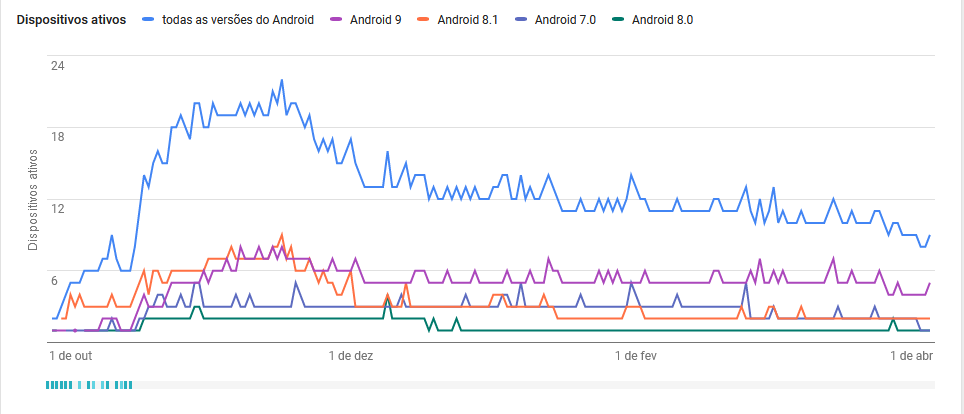
\includegraphics[scale=0.25]{Imagens/taxa_desocupacao.png}
\fonte{\citeonline{ibge_instituto_brasileiro_de_geografia_e_estatistica_pesquisa_2019}}
\label{figura_2}
\end{figure}


Com as universidades e institutos de ensino superior sendo reconhecidamente contextualizados como promotores da inovação no Brasil, país que configura o 13.º lugar entre os maiores produtores de publicações de pesquisa (\textit{papers}) e inovação a nível mundial, \citeonline{clarivate_analytics_web_of_research_2017}. 
O novo paradigma educacional, portanto, situa as instituições de ensino superior no campo da promoção do empreendedorismo direcional e sistemático, assim como o comportamento empreendedor, educação empreendedora disciplinada mostra-se eficaz no tocante ao surgimento das inovações, direcionadas e a promoção da identidade empreendedora para novos negócios, \cite{jain_academics_2009} já que a universidade vem a ser um local privilegiado do saber, da liberdade acadêmica e da experimentação científica tem o poder de ‘oficializar’ o empreendedorismo como um conteúdo de conhecimento é uma ferramenta capaz de gerar inovações \cite{dolabela_oficina_2008}. 

Já que o desenvolvimento do interesse ao empreendedorismo envolve diversos conteúdos de aprendizado, é necessário organizar as metodologias e suas aplicações pedagógicas \cite{rocha_avaliacao_2014}. O mesmo autor elencou os Principais Métodos, Técnicas e Recursos Pedagógicos no Ensino do Empreendedorismo. 


\begin{center}
\renewcommand\LTcaptype{quadro}
\begin{longtable}{p{3.5cm}p{11.0cm}}

\caption[\textbf{Principais  Métodos, Técnicas e Recursos Pedagógicos no Ensino de Empreendedorismo}]{\textbf{Principais  Métodos, Técnicas e Recursos Pedagógicos no Ensino de Empreendedorismo}} \label{tabela_2} \\


\hline \multicolumn{1}{p{3.5cm}}{\textbf{Métodos, Técnicas e Recursos}} & \multicolumn{1}{c}{\textbf{Aplicações}}\\ \hline 

\endfirsthead


\multicolumn{2}{c}%

{{\bfseries \quadroname \ \thequadro{} -\ \textbf{Continuação}}}\\

\hline \multicolumn{1}{p{3.5cm}}{\textbf{Métodos, Técnicas e Recursos}} & \multicolumn{1}{c}{\textbf{Aplicações}}  \\ \hline 

\endhead

\hline \multicolumn{2}{r}{{\textbf{Continua}}} \\ \hline

\endfoot
\hline \multicolumn{2}{r}{{\textbf{Continua}}} \\ \hline

\endfoot
\hline \multicolumn{2}{r}{{\textbf{Conclusão}}} \\ \hline
\hline \hline

\endlastfoot

Aulas expositivas & Transferir conhecimentos sobre o Empreendedorismo, as características pessoais do empreendedor, os processos de inovação, fontes de recursos, financiamentos e aspectos legais de pequenas empresas.  \\

Visitas e contatos com empresas & Estimular o \textit{network} e incitar o estudante a sair dos limites da IES para entender o funcionamento de mercado na vida real. Desenvolver visão de mercado.  \\

Plano de negócios & Desenvolver as habilidades de planejamento, estratégia, marketing, contabilidade, recursos humanos, comercialização. Desenvolver a habilidade de avaliação do novo negócio, analisando o impacto da inovação
no novo produto ou serviço. Construir habilidade de avaliar e dimensionar riscos do negócio pretendido. \\ 

Estudos de situações problemas & Construção da habilidade de pensamento crítico e de avaliação de cenários e
negócios. Desenvolver a habilidade de interpretação e definição de contextos associados ao Empreendedorismo. \\ 

Trabalhos teóricos em grupo & Construção da habilidade de aprender coletivamente. Desenvolver a
habilidade de pesquisar, dialogar, integrar e construir conhecimentos,
buscar soluções e emitir juízos de valor na realização do documento escrito. \\ 

Trabalhos práticos em grupo & Construção da habilidade de atuar em equipe. Desenvolver a habilidade de planejar, dividir e executar tarefas em grupo, de passar e receber críticas construtivas. Ampliar a integração entre o saber e o fazer.  \\ 

Grupos de discussão & Desenvolver a habilidade de testar novas ideias. Desenvolver a capacidade de avaliar mudanças e prospectá-las como fonte de oportunidades. \\ 
 
\textit{Brainstorming}  & Construção da habilidade de concepção de ideias, prospecção de
oportunidades, reconhecendo-as como oportunidades empreendedoras. \\ 


Seminários e palestras com empreendedores & Transferir conhecimentos das experiências vividas por empreendedores
desde a percepção e criação do produto, abertura do negócio, sucessos e
fracassos ocorridos na trajetória empreendedora. \\ 

Criação de empresa & Transpor as informações do plano de negócios e estruturar os contextos necessários para a formalização. Compreender várias etapas da evolução da empresa. Desenvolver a habilidade de organização e planejamento operacional. \\ 

Aplicação de provas dissertativas & Testar os conhecimentos teóricos dos estudantes e sua habilidade de
comunicação escrita. \\ 

Atendimento individualizado & Desenvolver a habilidade de comunicação, interpretação, iniciativa e
resolubilidade. Aproximar o estudante do cotidiano real vivido nos pequenos negócios. \\ 

Trabalhos teóricos individuais & Construção da habilidade de concepção de conhecimento individualizado,
estimulando a autoaprendizagem. Induzir o processo de autoaprendizagem. \\ 

Trabalhos práticos individuais & Construção da habilidade da aplicação dos conhecimentos teóricos
individuais, estimulando a autoaprendizagem. Estimular a capacidade
laboral e de auto realização. \\ 

Criação de produto & Desenvolver habilidade de criatividade, persistência, inovação e senso de
avaliação. \\ 

Filmes e vídeos & Desenvolver a habilidade do pensamento crítico e analítico, associando o
contexto assistido com o conhecimento teórico. Estimular a discussão em grupo e o debate de ideias. \\ 

Jogos de empresas e simulações & Desenvolver a habilidade de criar estratégias de negócios, solucionar
problemas, trabalhar e tomar decisões sob pressão. Aprender pelos próprios erros. Desenvolver tolerância ao risco, pensamento analítico, comunicação intra e intergrupais. \\ 

Sugestão de leituras & Prover ao estudante teoria e conceitos sobre o Empreendedorismo. Aumentar a conscientização do ato empreendedor. \\ 
Incubadoras & Proporcionar ao estudante espaço de motivação e criação da nova empresa, desenvolvendo múltiplas competências, tais como habilidades de liderança, organizacionais, tomada de decisão e compreender as etapas do ciclo de vida das empresas. Estimular o fortalecimento da network com financiadores, fornecedores e clientes. \\

Competição de planos de negócios & Desenvolver habilidades de comunicação, persuasão e estratégia.
Desenvolver capacidade de observação, percepção e aplicação de melhorias no padrão de qualidade dos planos apresentados. Estimular a abertura de empresas mediante os planos vencedores. \\ 

\end{longtable}
\fonte{\cite{rocha_avaliacao_2014}}
\renewcommand\LTcaptype{quadro}
\end{center}



Os centros de ensino devem contribuir para o desenvolvimento da “cultura empreendedora” por meio da “educação empreendedora” \cite{tscha_empreendendo_2014}, que incentive tanto Docentes quanto aos Discentes, deve incentivar “o despertarem dentro de si o espírito empreendedor e a explorar o espaço potencial para o empreendedorismo, transformando realidades por meio dos empreendimentos que podem desenvolver economicamente e socialmente um país e uma sociedade” \cite{tscha_empreendendo_2014}. Uma vez que, a cultura empreendedora depende diversos fatores influenciáveis ao longo do aprendizado e vida. \cite{dornelas_empreendedorismo:_2005} explica que  empreender segue fluxo um definido que depende de fatores determinantes durante a construção correta e satisfatória da cultura empreendedora. Alguns fatores estão descritos na figura \ref{figura_2}.

\begin{figure}[!htb]
\centering
\caption{\textbf{Fatores que influenciam o aprendizado do comportamento empreendedor:}}
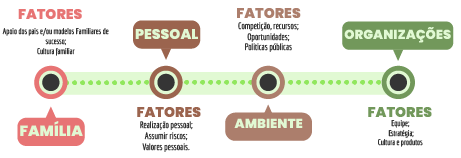
\includegraphics[scale=0.8]{Imagens/esquema_influencias_empreendedorismo.png}
\fonte{Adaptado de \cite{dornelas_empreendedorismo:_2005}}
\label{figura_2}
\end{figure}


Empreendedorismo acadêmico  apresenta-se também como uma potencial ferramenta para difusão e transferência de inovação e pesquisa por acadêmicos oriundos de laboratórios ou, departamentos onde a tecnologia se originou, \cite{guo_what_2019, abreu_nature_2013}, ou mesmo a busca de oportunidades e iniciativa utilizando os meios existentes no ambiente acadêmico. Os conteúdos necessários ao efetivo ensino do empreendedorismo vão além da oferta de apenas uma disciplina, é preciso que a instituição de ensino, a partir de novas práticas pedagógicas, transforme-se em também em uma instituição empreendedora \cite{campelli_empreendedorismo_2011}, que visualize a potencialidade da educação e promoção do comportamento empreendedor ao aluno com vistas a resolutividade de problemas \cite{degen_o_1989} e despertar da criatividade.

Diante da necessidade de solidificar o ensino empreendedor, que a \textit{Commission Enterprise and Industry Directorate-General} \cite{european_commission_best_2008} estruturou a educação empreendedora direcionada ao ensino superior em três objetivos, representados no modelo esquemático que pode ser visto na Figura \ref{figura_3}, em que se explica às três bases que estruturam os objetivos do ensino do Empreendedorismo no meio acadêmico. 

\begin{figure}[!htb]
\centering
\caption{\textbf{Pilares dos objetivos do ensino ao empreendedorismo.}}
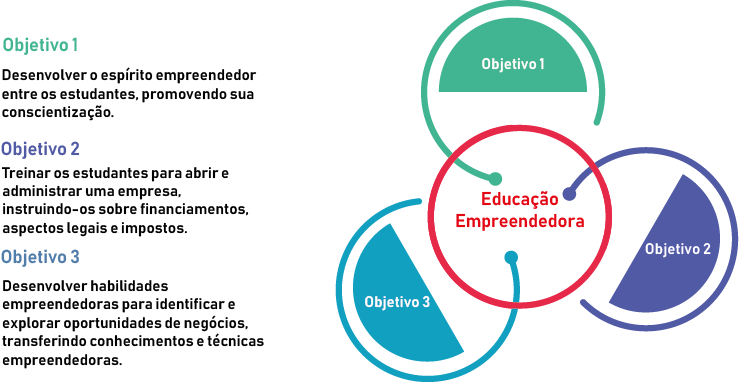
\includegraphics[scale=0.8]{Imagens/figura2.png}
\fonte{Adaptado de \cite{european_commission_best_2008}}
\label{figura_3}
\end{figure}
\newpage

Como visto, ensino do empreendedorismo perpassa por diversas vertentes, porém, visando a associação de tais conteúdos aos técnicos científicos de forma interdisciplinar, e explorado neste trabalho a proposta de educação empreendedora que tem como base a Aprendizagem Baseada em Problemas (ABPR), a Aprendizagem Baseada em Projetos (ABP) \cite{bender_aprendizagem_2015} tendo como passos para elaboração dos conteúdos para o desenvolvimento de um empreendimento bem-sucedido os passos de \cite{aulet_empreendedorismo_2019} no livro: Empreendedorismo Disciplinado. 
Segundo \cite{bender_aprendizagem_2015} a ABP tem como objetivo o desenvolvimento do autoconhecimento com ênfase na perseverança, na imaginação, na criatividade, na inovação, para resolubilidade de problemas reais, sendo um importante o conteúdo que se aprende a fazer, mas, sobretudo, o que aprendido \cite{souza_disseminacao_2001}, de forma que a união de tais conhecimentos se some a um melhor desenvolvimento aos profissionais graduados que irão ao mercado de trabalho ou ao mundo dos negócios. Já que conhecimento científico promovido de forma interdisciplinar na graduação, além de repassar os conhecimentos técnicos, promove  uma considerável contribuição para se desenvolver o raciocínio independente, criativo e inovador buscamos neste trabalho uma abordagem que possa explorar todos os conteúdos de uma metodologia disciplinada e estruturada.


\section{Propriedade Intelectual no meio rural}

Toda criação advinda do intelecto humano, tais como música, produto, processo, nova cultivar, desenhos, artigos científicos, trabalhos literários ou artísticos constituem um ativo, bem ou direito \cite{costa_interseccao_2011}. Tais ativos sendo eles registrados ou não estão ligados diretamente ao seu autor/inventor sendo a propriedade  intelectual. Este direito vai muito além da inovação em si \cite{wipo_tratado_1970}, mas a relação entre o seu autor/inventor e sua respectiva criação intelectual. 


O conceito de Propriedade Intelectual é amplo e difere de país a país, em suma pode ser entendido como, à área do Direito que, garante a inventores ou responsáveis por qualquer produção do intelecto, seja nos domínios industrias, científicos, literários ou artísticos, o direito de obter, por um determinado período de tempo, recompensa pela própria criação \cite{aspi_aspi_2019}, é amparo legal e necessário para garantir que os investimentos em pesquisa e desenvolvimento retornem ao inventor, provocando um processo cíclico positivo, em que maiores investimentos em P&D seriam promovidos diante da concessão do monopólio temporário de exploração do invento \cite{lima_sauglobal_2017}. No Brasil a PI é composta por três grandes áreas: Propriedade Industrial, Direito do Autor e Suis generis, demais ramificações podem ser vistas na figura \ref{figura_4}.


\begin{figure}[h!]
\centering
\caption{\textbf{Modalidades da propriedade intelectual no Brasil}}
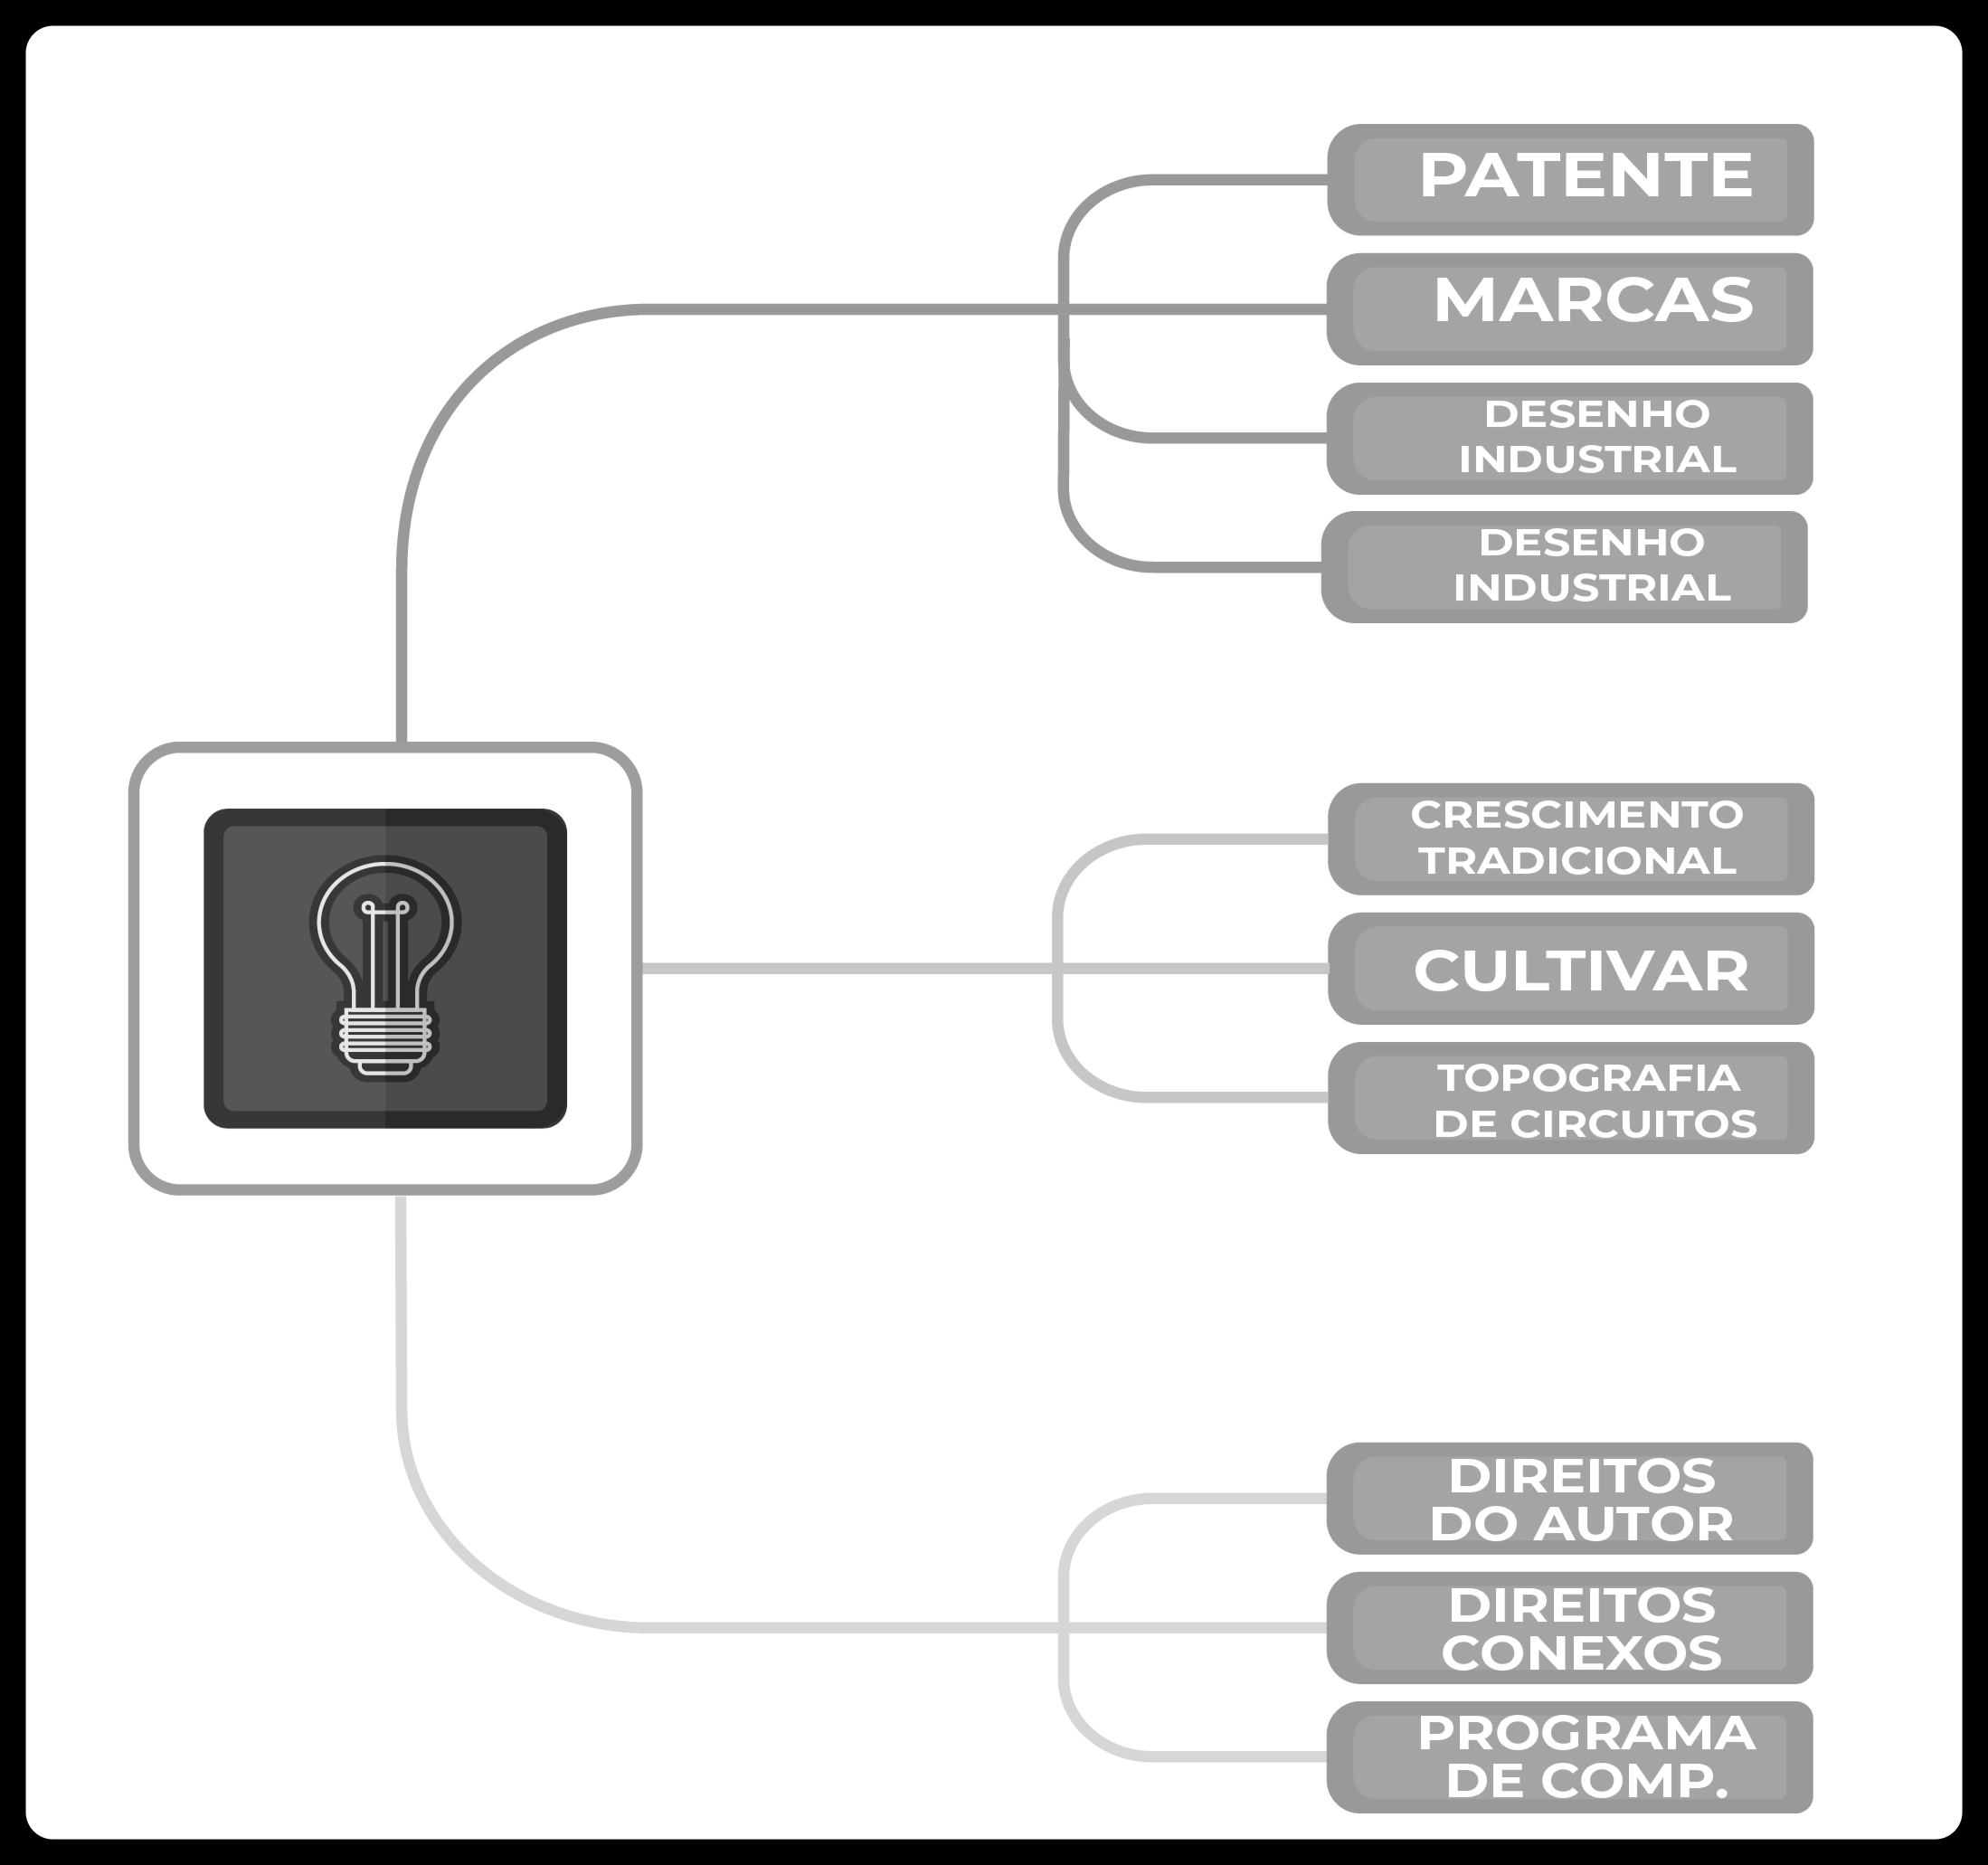
\includegraphics[scale=0.75]{Imagens/propriedade_intelectual.png}
\fonte{Adaptado de \cite{inpi_manual_2017}}
\label{figura_4}
\end{figure}


Aliadas  às  ações  para  o  desenvolvimento  de  inovações, o inventor ou autor deve ter certa atenção as Propriedades Intelectuais que tangem seu produto, ou processo.  Sendo assim, é visível que há uma grande afinidade entre estes dois temas, principalmente os direitos que cabe ao meio industrial e do autor ligados a software. 

A crescente interação comercial,  financeira  e  tecnológica  entre  a  economia  e  seus  agentes  exigem  padrões  modernos  de  proteção  para  a  PI,  uma  vez  que  os  direitos sobre os nomes empresariais, tecnologias, \textit{designs}, marcas, entre outros, representam valiosos ativos das empresas e profissionais autores/inventores \cite{sherwood_propriedade_1992}. 


Diante de tais mudanças sobre o cenário do desenvolvimento tecnológico e das Propriedades Intelectuais (PI) inúmeras questões sobre o papel que os sistemas de registro e divulgação para PI desempenham no desenvolvimento e o incentivo à inovação \cite{segala_os_2016}. Os países que apresentam uma economia mais forte, dispõe de um sistema de proteção de propriedade mais robusto e confiável, concomitantemente, uma maior quantidade de registros e depósitos das mais variadas finalidades \cite{mueller_universidades_2014}.



